\chapter{Análise da Participação das Aposentadorias e Pensões na Distribuição de Renda do Brasil, 2000 e 2010}

% --------------------------------------------------------------------------- %
\section{Considerações Iniciais}

A distribuição de renda, ou distribuição de riquezas, de um país é um tópico de inquestionável importância em todos os seguimentos da sociedade devido, principalmente, ao fato de estar diretamente relacionado com as condições de vida da população. Tal assunto apresenta-se em constante evidencia no cenário brasileiro uma vez que esse apresenta-se como um dos países mais desiguais do mundo \cite{cap04_ref2, cap04_ref3}. De acordo com dados da \cite{cap04_ref1}, o Brasil ocupa a 156ª posição\footnote{Não há dados atualizados de índice de Gini em diversos países, indicando dessa forma que, possivelmente, o Brasil não ocupe exatamente a posição informada.}  no ranking de índices de Gini de mundo, corroborando para que grande parte da população nacional tenha rendimentos insuficientes para atender suas necessidades básicas.

Entretanto, informações anuais divulgadas pela PNAD revelam que a desigualdade de renda nacional sofreu uma substancial redução nos últimos anos \cite{cap04_ref4} - ainda que se apresente muito elevada comparada a outros países do mundo. Paralelamente a esse fator, outros indicadores do mercado de trabalho, como taxas de informalidade e desemprego, demonstram-se regressivos nos últimos anos, apontando uma possível contribuição para a diminuição do índice de Gini registrado. A Figura~\ref{fig:cap04:gini_taxas} ilustra o comportamento dessas métricas no Brasil entre os anos de 2001-2014.

\begin{figure}[!h]
    \centering
    \caption{Variação das taxas de formalidade e fesemprego e do índice de Gini no Brasil, 2001 a 2014}
    \includegraphics[width=0.8\textwidth]{figs/cap04_gini_taxas.pdf}
    \caption*{\footnotesize{Fonte: Elaborado pelo autor a partir de dados contidos em  \cite{cap04_ref4}}}
    \label{fig:cap04:gini_taxas}
\end{figure}

Paralelamente, os benefícios de aposentadorias e pensões compreendem uma importante parcela de rendimento da população, apresentando-se cada vez mais ativos na composição de renda dos domicílios brasileiros \cite{cap02_ref22, cap04_ref5}. Esses benefícios, em sua grande maioria, correspondem a repasses garantidos pela Previdência Social, objetivando assegurar o rendimento dos contribuintes quando esses não detêm mais de suas capacidades laborais \cite{cap04_ref6}.

Diante desse fator, oberava-se na literatura uma divergência de pontos de vista relacionados a contribuição dessa parcela de benefícios para o aumento ou diminuição da distribuição de renda no Brasil. Alguns trabalhos como \cite{cap04_ref7, cap04_ref8, cap04_ref9} indicam que as aposentadorias e pensões colaboram para o crescimento do coeficiente de Gini tanto em escala nacional quanto regional. No entanto, as pesquisas de \cite{cap04_ref10, cap04_ref11} demonstram que essa parcela de benefícios colabora para a redução da desigualdade de renda no Brasil.

Revisando o estado da arte relacionado a essa problemática, nota-se que grande parte dos estudos abstraem seus \textit{insights} a partir dos microdados anuais divulgados pela PNAD. Entretanto, tal estratégia restringe as possibilidades de avaliações a serem realizadas em virtude dessa pesquisa corresponder a uma amostra domiciliar efetuada nas unidades federativas brasileiras, impossibilitando a flexibilidade para análises em unidades territoriais menores como municípios ou setores censitários. Uma avaliação municipal da proporcionalidade entre a distribuição de renda e os repasses de aposentadorias e pensões, apresenta-se como uma importante forma de compreender o real impacto que esses benefícios causam no coeficiente de Gini nacional. Tal importância destaca-se no trabalho de \cite{cap04_ref12}, o qual compreende a previdência social como instrumento assistencial que combate à pobreza em diversos municípios brasileiros.

Diante disso, neste estudo de caso é realizada uma avaliação da participação que os rendimentos de aposentadorias e pensões tem na distribuição de riquezas dos estados e municípios do Brasil. Para tanto, optou-se por utilizar estratégias e conceitos de ciência de dados acerca dos microdados dos censos demográficos de 2000 e 2010, e a metodologia de decomposição do índice de Gini - conforme descrito no capítulo ~\ref{cap:referencias} - para aferir o grau de contribuição das parcelas desejadas.

Dessa forma, esse capítulo foi dividido em 4 subseções incluindo esta introdução. Na subseção~\ref{cap04:metodologia}, será abordada a metodologia utilizada para o desenvolvimento das análises propostas, demonstrando detalhadamente os tratamentos e processamentos efetuados acerca dos dados. Na subseção~\ref{cap04:resultados} serão discutidos os principais resultados encontrados, finalizando o estudo na subseção~\ref{cap04:conclusoes} com as considerações finais. 

\section{Metodologia Utilizada}\label{cap04:metodologia}

O procedimento metodológico para a realização do estudo proposto foi sistematizado mediante a uma sequência de etapas de análise de dados: extração, pré-processamento, aplicação de modelos matemáticos/computacionais e abstração de informações acerca dos dados de entrada. A Figura~\ref{fig:cap04:metodologia} ilustra o fluxograma de desenvolvimento do trabalho contendo cada uma das etapas realizadas, havendo um maior grau de detalhamentos acerca destas no decorrer dessa subseção. 

\begin{figure}[!h]
    \centering
    \caption{Fluxograma de desenvolvimento do primeiro estudo de caso}
    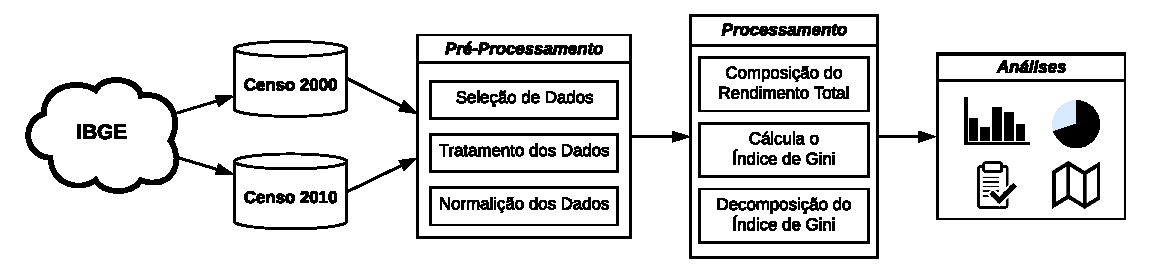
\includegraphics[width=\textwidth]{figs/cap04_metodologia_estudo01.pdf}
    \caption*{\footnotesize{Fonte: Elaborado pelo autor}}
    \label{fig:cap04:metodologia}
\end{figure}

% --------------------------------------------------------------------------- %

\subsection{Origem dos Dados}

Os microdados utilizados na execução das análises desse estudo foram extraídos dos censos demográficos realizados pelo IBGE nos anos de 2000 e 2010. As informações referentes aos censos anteriores, como por exemplo 1991, foram desconsiderados na pesquisa devido aos altos índices de inflação recorrentes na época \cite{cap04_ref13}, gerando por consequência baixa confiabilidade nos resultados gerados.

O censo demográfico brasileiro trata-se de uma pesquisa nacional realizada cada dez anos, visando o reconhecimento das condições de vida da população brasileira em todas as grandes regiões, unidades federativas, mesorregiões, microrregiões, regiões metropolitanas, municípios, distritos, subdistritos e setores censitários, tendo como objeto de coleta as pessoas residentes (na data de referência) em domicílios presentes no território nacional \cite{cap04_ref14}. No site do censo\footnote{Disponível em: <https://www.ibge.gov.br/estatisticas/sociais/populacao/9662-censo-demografico> Acesso em: 20 Dez, 2019} é possível encontrar os principais resultados, estatísticas, tabelas e publicações realizadas pelo IBGE. Entretanto, o instituto também fornece os microdados e documentação referentes a cada pesquisa realizada, possibilitando que a comunidade acadêmica, empresas ou até mesmo pessoas físicas realizem pesquisas acerca destes. 

Os microdados disponibilizados pelas bases são divididos em 3 grupos de informações, os quais abrangem pessoas, famílias e domicílios. Essa classificação possibilita estudos estatísticos acerca de qualquer uma dessas categorias de forma isolada, permitindo análises com alto grau de detalhamento, dependendo da dimensão da problemática em questão. O presente trabalho norteou-se a partir das classes pessoas e domicílios, com recortes espaciais para as unidades federativas e municípios brasileiros. 

O censo demográfico difere-se da PNAD, principalmente, em abrangência territorial e quantidade de informações exploradas. Enquanto a primeira pesquisa realiza uma investigação profunda em todo território nacional sobre as características socioeconômicas\footnote{Resumidamente, o censo demográfico aborda os seguintes temas: características dos domicílios, identificação étnico-racial, nupcialidade, núcleo familiar, religião, deficiência, migração, educação, trabalho, rendimento e mortalidade.} da população, a segunda propõe uma apuração domiciliar mais limitada\footnote{Os temas abordados na PNAD são: habitação, características gerais dos moradores, características do trabalho, rendimentos e educação.}, restringindo apenas ao grau de representatividade necessária para os seus resultados acerca dos diversos níveis geográficos\footnote{A PNAD abrange o Brasil, Grandes Regiões, Unidades da Federação, Regiões Metropolitanas que contêm Municípios das Capitais, Municípios das Capitais e Região Integrada de Desenvolvimento da Grande Teresina.} definidos na sua divulgação.

\subsection{Pré-Processamento dos Dados}

Os censos demográficos foram carregados em um Sistema Gerenciador de Banco de Dados (SGBD) objetivando facilitar as consultas acerca dos microdados em questão. Constatou-se que a base de dados do ano 2000 possuía mais de 280 variáveis relacionadas à domicílios, famílias e pessoas, e que a de 2010 ultrapassava 350 variáveis correspondentes a domicílios, pessoas, mortalidade e emigração. Dessa forma, foi realizada uma etapa preliminar de seleção de atributos com o intuito de filtrar somente as informações de interesse para as posteriores análises. A Tabela~\ref{tab:cap04:variaveis} exibe as 7 variáveis utilizadas no presente estudo e suas respectivas descrições.
	
\begin{table}[!h]
    \centering
    \caption{Variáveis selecionadas dos censos demográficos e suas descrições} 
    \begin{tabular}{|p{2cm}|p{2cm}|p{10cm}|}
        \hline
        \multicolumn{2}{|c|}{\textbf{Código das Variáveis}} & \multicolumn{1}{c|}{\multirow{2}{*}{\textbf{Descrição}}} \\ \cline{1-2}
        \centering\textbf{2000} & \centering\textbf{2010} & \multicolumn{1}{c|}{} \\ \hline
        \centering v0102 & \centering v0001 & Código do estado \\ \hline
        \centering v0103 & \centering v0002 & Código do município \\ \hline
        \centering v7616 & \centering v6529 & Rendimento mensal domiciliar \\ \hline 
        \centering v4614 & \centering v6527 & Rendimento mensal per capita \\ \hline
        \centering v4573 & \centering v6591 & Rendimento dos benefícios de aposentadorias e pensões \\ \hline
        \centering - & \centering v0656 & Aposentadorias e pensões da Previdência Social \\ \hline
        \centering p001 & \centering v0010 & Peso de cada registro\\ \hline
    \end{tabular}
    \caption*{\footnotesize{Fonte: Elaborado pelo autor a partir dos metadados dos censos demográficos de 2000 e 2010}}
    \label{tab:cap04:variaveis}
\end{table}

A seleção dessas variáveis norteou-se com base nas informações necessárias para mensurar o grau de desigualdade e calcular a decomposição do índice de Gini (conforme demonstrado na subseção~\ref{cap:referencias:gini}) acerca das unidades territoriais de interesse.  Observando a Tabela~\ref{tab:cap04:variaveis}, nota-se a presença de um atributo extra na base do censo demográfico do ano de 2010, tal fator é explicado pela necessidade de uma variável auxiliar para designar a qual programa social cada benefício pertence. Adicionalmente foram utilizados os valores de salário mínimo registrados nos meses de abril de ambos os anos abordados, sendo 151 e 510 reais para 2000 e 2010 respectivamente.

Posteriormente, foi realizada uma etapa de tratamento de dados objetivando corrigir erros e possíveis inconsistências existentes nas bases. Devido ao fato de ser uma pesquisa com elevado grau de importância e responsabilidade, foram identificadas poucas anomalias que comprometessem as análises realizadas. No entanto, foi necessária a substituição dos dados ausentes de rendimentos de aposentadorias e pensões por valores zeros (casos específicos de pessoas que não gozavam desses benefícios) e a correção dos pesos que apresentavam escalas erradas em estados e cidades especificas. 

Além disso, em decorrência do elevado dinamismo da malha territorial brasileira \cite{cap04_ref17}, constatou-se uma divergência no número de municípios existente em cada base de dados, registrando 5.507 cidades para o ano de 2000 e 5.564 para 2010. Dessa forma, houve a necessidade de normalizar o número de cidades para ambos os anos adotando como estratégia a criação de Área Mínimas Comparáveis (AMC), as quais são definidas como sendo áreas geográficas com a máxima unidade territorial desagregada, possibilitando dessa forma a comparação entre dois pontos diferentes no tempo \cite{cap04_ref15, cap04_ref16}. Sendo assim, define-se cada AMC como:

\begin{equation}
    AMC(p, r, b, w) = \sum_{i}^{n} mun_{i}(p, r, b, w), \{\forall n \in N\}
\end{equation}

\noindent onde, $p$ corresponde à população, $r$ aos rendimentos, $b$ os valores dos benefícios de aposentadorias e pensões e $w$ os pesos de cada município $n$. Sendo $N$ cada subconjunto de municípios que foram desmembrados em relação aos originais do ano 2000.

% --------------------------------------------------------------------------- %

\subsection{Processamento}

Após a realização dos estágios de seleção, tratamento e normalização dos microdados, foi possível efetuar a etapa de processamento, sendo essa responsável por mensurar os valores do coeficiente de Gini, o percentual de participação das aposentadorias e pensões e o impacto que esses benefícios causam na distribuição de renda da população acerca das unidades territoriais de interesse Para isso, foi adotada a metodologia abordada na subseção~\ref{cap:referencias:gini}, utilizando como parâmetros das equações as variáveis contidas na Tabela~\ref{tab:cap04:parametros}.  

\begin{table}[!ht]
    \centering
    \caption{Parâmetros de indexação e notação geral.} 
    \begin{tabular}{|c|c|c|}
        \hline
        Variável & Significado                & Valor                                 \\ \hline
        k        & estado                     & São Paulo, Rio de Janeiro, Pará, etc. \\ \hline
        i        & cidade                     & Fortaleza, Belém, Curitiba, etc.      \\ \hline
        r        & renda per capita           & R\$ 0, ... , R\$ 1.000, ...           \\ \hline
        d        & renda domiciliar           & R\$ 0, ... , R\$ 1.000, ...           \\ \hline
        b        & renda aposentadoria/pensão & R\$ 0, ... , R\$ 1.000, ...           \\ \hline
        s        & salário mínimo             & R\$ 151 ou R\$ 510                    \\ \hline
        t        & ano                        & 2000 ou 2010                          \\ \hline
        p        & peso                       & 0, ... , 0.01, ... , 1.10, ...        \\ \hline
    \end{tabular}
    \caption*{\footnotesize{Fonte: Elaborado pelo autor.}}
    \label{tab:cap04:parametros}
\end{table}

Para o cálculo do índice de Gini optou-se por utilizar a renda per capita domiciliar conforme é retratado na literatura \cite{cap02_ref22, cap04_ref10, cap04_ref11, cap04_ref8, cap04_ref1, cap02_ref2}. Dessa forma, o grau de desigualdade dos estados e municípios brasileiros ($Desigualdade$) pode ser interpretado pela Equação~\ref{eq:4.2}, sendo: 

\begin{equation}\label{eq:4.2}
    Desigualdade(t, k, i) = Gini(t, k, i, d, p), \{\forall d > 0\}
\end{equation}

\noindent onde $Desigualdade$ corresponde ao coeficiente de Gini, dos domicílios com rendimento, para cada município $i$ e estado $k$ nos anos $t$, conforme descrito em \ref{eq:2.6}.

Posteriormente, para mensurar o grau de participação das aposentadorias e pensões na composição de renda da população, calculou-se o quociente entre os valores desses benefícios e o total de rendimentos per capita de cada unidade territorial $k$ e $i$, e ano $t$. Dessa forma, pode-se entender o grau de participação ($PartBeneficio$) como sendo: 

\begin{equation}
    PercBeneficios(t, k, i) = \dfrac{\mathlarger{\sum_{N}} \ b(n, p, t, k, i)}{\mathlarger{\sum_{M}} \ r(m, p, t, k, i)}, \{n \subset N \And m \subset M\}
\end{equation}

\noindent sendo $N$ e $M$ os conjuntos universos de valores de renda de aposentadorias/pensões e rendimentos per capita, respectivamente.

Por fim, aferiu-se o impacto que esses benefícios de aposentadorias e pensões causam acerca da variável $Desigualdade$ utilizando a metodologia de decomposição do índice de Gini para cada cidade $i$ e estado $k$ nos anos $t$, semelhante a equação~\ref{eq:4.2}. Sendo assim, estimou-se a razão concentração ($Concentracao$) desses benefícios como:

\begin{equation}\label{eq:4.4}
    Concentracao (t, k, i) = C_h(t, k, i, b, p), \{\forall b > 0\}
\end{equation}

\noindent onde $C_h$ corresponde a Equação descrita em \ref{eq:2.10}. 

Dessa forma, a medida de progressividade ($\pi$) pode ser compreendida por:

\begin{equation}\label{eq:4.5}
    \pi(t, k, i) = Desigualdade(t, k, i) - Concentracao (t, k, i)
\end{equation}

Paralelamente, utilizando os conceitos das Equações~\ref{eq:4.4} e \ref{eq:4.5}, calculou-se também as medidas de progressividade para os benefícios até 1 salário mínimo e acima de 1 salário mínimo acerca de cada unidade salarial $s$. 

Para a realização dos cálculos propostos, foi utilizada a linguagem de programação \textit{Python 3}\footnote{Disponível em: <https://www.python.org/> Acesso em: 05 Jan, 2020}, devido a sua facilidade para trabalhar com grandes volumes de dados, e as bibliotecas de análise dados \textit{Pandas}\footnote{Disponível em: <https://www.pandas.pydata.org/> Acesso em: 05 Jan, 2020}, \textit{Numpy}\footnote{Disponível em: <https://www.numpy.org/> Acesso em: 05 Jan, 2020} e \textit{Scikit-Learn}\footnote{Disponível em: <https://www.scikit-learn.org/stable/> Acesso em: 05 Jan, 2020}. Além disso, foi utilizado o \textit{software} QGIS 2.18\footnote{Disponível em: <https://www.qgis.org/pt\_BR/site/> Acesso em: 05 Jan, 2020} para a elaboração de mapas temáticos objetivando proporcionar uma melhor visualização acerca dos resultados encontrados. O projeto está disponibilizado na plataforma do GitHub\footnote{Disponível em: <https://github.com/jralbbuquerque/censo-beneficio> Acesso em: 05 Jan, 2020} sob uma licença GNU \textit{General Public License} (GPL) v3.0, contendo todo o procedimento para a reprodução das análises realizadas, tais como documentação, \textit{scripts}, arquivos e referências necessárias para que a sua replicação e possíveis contribuições possam ser realizadas pela comunidade científica. A Tabela~\ref{tab:cap04:github} descreve a estrutura do projeto e os principais arquivos existentes.

\newpage

\begin{table}[h]
    \centering
    \caption{Descrição dos principais arquivos do projeto no GitHub referente ao primeiro estudo de caso} 
    \begin{tabular}{p{0.22\textwidth}p{0.6\textwidth}}
    \hline
    \textbf{requirements.txt} & arquivo de texto descrevendo todas as dependências e pacotes Python necessários para a execução do projeto.\vspace{3mm}            \\
    \textbf{dataset}          & pasta na qual serão salvos todos os resultados (arquivos .xlsx) da execução do projeto.\vspace{3mm}                                \\
    \textbf{datasrc}          & pasta contendo todos os dados necessários para a execução das análises.\vspace{3mm}                                                \\
    \textbf{util}             & pasta com os diversos módulos/métodos para os cálculos dos indicadores.\vspace{3mm}                                                \\
    \textbf{metadata}         & pasta contendo os dicionários e documentações das bases de dados, disponibilizados no site do IBGE.\vspace{3mm}                    \\
    \textbf{maps}             & pasta com os arquivos e dados de entrada do software QGIS necessários para a elaboração dos mapas.\vspace{3mm}                     \\
    \textbf{analisys}         & pasta com as diversas análises realizadas utilizando a \textit{framework jupyter notebook}.\vspace{3mm}                                     \\
    \textbf{main.py}          & arquivo principal para a execução do projeto.\vspace{3mm}                                                                          \\
    \textbf{README.md}        & descrição do funcionamento do projeto.
    \\\hline
    \end{tabular}
    \caption*{\footnotesize{Fonte: Elaborado pelo autor.}}
    \label{tab:cap04:github}
\end{table}

\newpage
% --------------------------------------------------------------------------- %
\section{Resultados e Discussões}\label{cap04:resultados}

O Rendimento Domiciliar per capita (RD), utilizado para os cálculos do trabalho, é referente a renda total, soma de todas as parcelas investigadas nos censos demográficos, dos domicílios registrados nas bases de dados. Diante disso, a Tabela~\ref{tab:cap04:giniestados} exibe os valores de índice de Gini (G) dos estados brasileiros em 2000 e 2010, e seus respectivos valores de renda média per capita. Nesta também é possível verificar as variações ocorridas entre os anos investigados, possibilitando uma visualização nas alterações de distribuições de renda dos estados brasileiros para o intervalo analisado. Os dados equivalentes a renda mensal de 2000 foram convertidos para a mesma unidade monetária de 2010, levando em consideração o Índice Nacional de Preços ao Consumidor (INCP), deflacionando todos os valores para outubro de 2010.

\begin{table}[!h]
    \caption{Índice de Gini (G) e renda média domiciliar (RD), Brasil 2000 e 2010.} 
    \resizebox{\textwidth}{!}{
    \renewcommand{\arraystretch}{1.15}
    \begin{tabular}{lccccccccc}
    \Xhline{2pt}
     & AC & AL & AM & AP & BA & CE & DF & ES & GO \\ \cline{2-10} 
    Gini (G) - 2000 & 0,6233 & 0,6615 & 0,6470 & 0,6126 & 0,6437 & 0,6537 & 0,6226 & 0,5947 & 0,6164 \\
    Gini (G) - 2010 & 0,6133 & 0,6087 & 0,6355 & 0,5924 & 0,6071 & 0,5996 & 0,6185 & 0,5632 & 0,5603 \\
    Variação Gini ($\Delta$\%) & {\color[HTML]{FE0000} -1,61\%} & {\color[HTML]{FE0000} -7,98\%} & {\color[HTML]{FE0000} -1,77\%} & {\color[HTML]{FE0000} -3,29\%} & {\color[HTML]{FE0000} -5,70\%} & {\color[HTML]{FE0000} -8,28\%} & {\color[HTML]{FE0000} -0,67\%} & {\color[HTML]{FE0000} -5,30\%} & {\color[HTML]{FE0000} -9,10\%} \\
    RD (R\$) - 2000 & 1521,24 & 1190,33 & 1669,78 & 1978,99 & 1291,75 & 1295,35 & 4376,14 & 2088,34 & 2003,57 \\
    RD (R\$) - 2010 & 1875,25 & 1533,41 & 2182,59 & 2419,99 & 1626,95 & 1576,03 & 5393,59 & 2496,47 & 2456,14 \\
    Variação RD ($\Delta$\%) & {\color[HTML]{00009B} 23,27\%} & {\color[HTML]{00009B} 28,82\%} & {\color[HTML]{00009B} 30,71\%} & {\color[HTML]{00009B} 22,28\%} & {\color[HTML]{00009B} 25,95\%} & {\color[HTML]{00009B} 21,67\%} & {\color[HTML]{00009B} 23,25\%} & {\color[HTML]{00009B} 19,54\%} & {\color[HTML]{00009B} 22,59\%} \\ \Xhline{2pt}
     & MA & MG & MS & MT & PA & PB & PE & PI & PR \\ \cline{2-10} 
    Gini (G) - 2000 & 0,6390 & 0,6035 & 0,6221 & 0,6281 & 0,6311 & 0,6285 & 0,6527 & 0,6425 & 0,5976 \\
    Gini (G) - 2010 & 0,6071 & 0,5565 & 0,5605 & 0,5636 & 0,6032 & 0,5982 & 0,6195 & 0,6041 & 0,5384 \\
    Variação Gini ($\Delta$\%) & {\color[HTML]{FE0000} -4,99\%} & {\color[HTML]{FE0000} -7,80\%} & {\color[HTML]{FE0000} -9,91\%} & {\color[HTML]{FE0000} -10,27\%} & {\color[HTML]{FE0000} -4,41\%} & {\color[HTML]{FE0000} -4,83\%} & {\color[HTML]{FE0000} -5,09\%} & {\color[HTML]{FE0000} -5,98\%} & {\color[HTML]{FE0000} -9,91\%} \\
    RD (R\$) - 2000 & 992,43 & 2027,05 & 2051,77 & 2137,66 & 1552,25 & 1196,18 & 1447,89 & 1088,33 & 2244,49 \\
    RD (R\$) - 2010 & 1375,88 & 2337,88 & 2459,68 & 2378,52 & 1725,3 & 1588,88 & 1729,64 & 1487,87 & 2707,04 \\
    Variação RD ($\Delta$\%) & {\color[HTML]{00009B} 38,64\%} & {\color[HTML]{00009B} 15,33\%} & {\color[HTML]{00009B} 19,88\%} & {\color[HTML]{00009B} 11,27\%} & {\color[HTML]{00009B} 11,15\%} & {\color[HTML]{00009B} 32,83\%} & {\color[HTML]{00009B} 19,46\%} & {\color[HTML]{00009B} 36,71\%} & {\color[HTML]{00009B} 20,61\%} \\ \Xhline{2pt}
     & RJ & RN & RO & RR & RS & SC & SE & SP & TO \\ \cline{2-10} 
    Gini (G) - 2000 & 0,5964 & 0,6393 & 0,6022 & 0,6036 & 0,5774 & 0,5539 & 0,6396 & 0,5834 & 0,6411 \\
    Gini (G) - 2010 & 0,5955 & 0,5931 & 0,5669 & 0,6158 & 0,5400 & 0,4918 & 0,6110 & 0,5632 & 0,5949 \\
    Variação Gini ($\Delta$\%) & {\color[HTML]{FE0000} -0,14\%} & {\color[HTML]{FE0000} -7,23\%} & {\color[HTML]{FE0000} -5,86\%} & {\color[HTML]{FE0000} 2,01\%} & {\color[HTML]{FE0000} -6,49\%} & {\color[HTML]{FE0000} -11,20\%} & {\color[HTML]{FE0000} -4,47\%} & {\color[HTML]{FE0000} -3,46\%} & {\color[HTML]{FE0000} -7,21\%} \\
    RD (R\$) - 2000 & 2730,73 & 1428,89 & 1808,49 & 1934,10 & 2334,21 & 2438,09 & 1306,36 & 3065,76 & 1384,11 \\
    RD (R\$) - 2010 & 2980,77 & 1849,94 & 2145,43 & 2194,02 & 2734,68 & 2984,14 & 1754,60 & 3278,10 & 1955,62 \\
    Variação RD ($\Delta$\%) & {\color[HTML]{00009B} 9,16\%} & {\color[HTML]{00009B} 29,47\%} & {\color[HTML]{00009B} 18,63\%} & {\color[HTML]{00009B} 13,44\%} & {\color[HTML]{00009B} 17,16\%} & {\color[HTML]{00009B} 22,40\%} & {\color[HTML]{00009B} 34,31\%} & {\color[HTML]{00009B} 6,93\%} & {\color[HTML]{00009B} 41,29\%} \\ \Xhline{2pt}
    \end{tabular}}
    \label{tab:cap04:giniestados}
    \caption*{\footnotesize{Fonte: Elaborado pelo autor.}}
\end{table}

É possível observar uma redução no índice de Gini para todos os estados, evidenciando uma diminuição na concentração de renda em todo o território brasileiro, com um decréscimo no indicador de aproximadamente -5,59\% em escala nacional. Destacam-se positivamente os estados de Goiás (GO), Mato Grosso (MT), Mato Grosso do Sul (MS), Santa Catarina (SC) e Paraná (PR) com uma redução percentual acima de 9\% para o índice. Além disso, houve um evidente acréscimo nas rendas médias domiciliares estaduais, com variação percentual média de aproximadamente +22,84\%, fator essencial e determinante para a redução da desigualdade indicada pelo coeficiente de Gini.

Ainda que haja uma evidente melhora na redução do coeficiente de Gini para o período analisado em todo território brasileiro, é notória a heterogeneidade de concentração de renda existente entre os estados. Por exemplo, em 2010 foram reportados índices de Gini para o Brasil e Argentina de aproximadamente 0,525 e 0,430 respectivamente, contabilizando uma diferença em torno de 0,095 entre os países \cite{cap04_ref1}. Ao realizarmos a mesma análise nos estados do Amazonas (AM) e de Santa Catarina (SC), observamos uma diferença de 0,144 para ano de 2010 (valor acima da diferença dos índices de Gini entre Brasil e Argentina), evidenciando que a dispersão encontrada entre os estados brasileiro é equivalente a existente entre países com economias distintas \cite{cap04_ref11}.

Na Figura~\ref{fig:cap04:ginicidades} é ilustrada a situação do coeficiente de Gini no Brasil com recorte geográfico para cidades e seus rendimentos médios domiciliares. Nas subfiguras \ref{fig:cap04:ginicidades}(a) e \ref{fig:cap04:ginicidades}(b) são exibidas as dispersões da variável acerca dos municípios nos anos de 2000 e 2010 respectivamente, enfatizando a evidente diminuição do parâmetro. Destacam-se positivamente as regiões Centro-Oeste, Sul, Nordeste e Sudeste com consideráveis reduções municipais no indicador. Embora tenha ocorrido uma redução na concentração de renda dos estados e cidades brasileiras, é importante salientar que os valores calculados permaneceram bem acima do desejado quando comparados a maioria dos países europeus e asiáticos ($G < 0,40$) \cite{cap04_ref1}.

\begin{figure}[!ht]
    \centering
    \caption{(a) e (b): Índice de Gini das cidades brasileiras. (c) e (d): Rendimento médio domiciliar dos municípios brasileiros}
    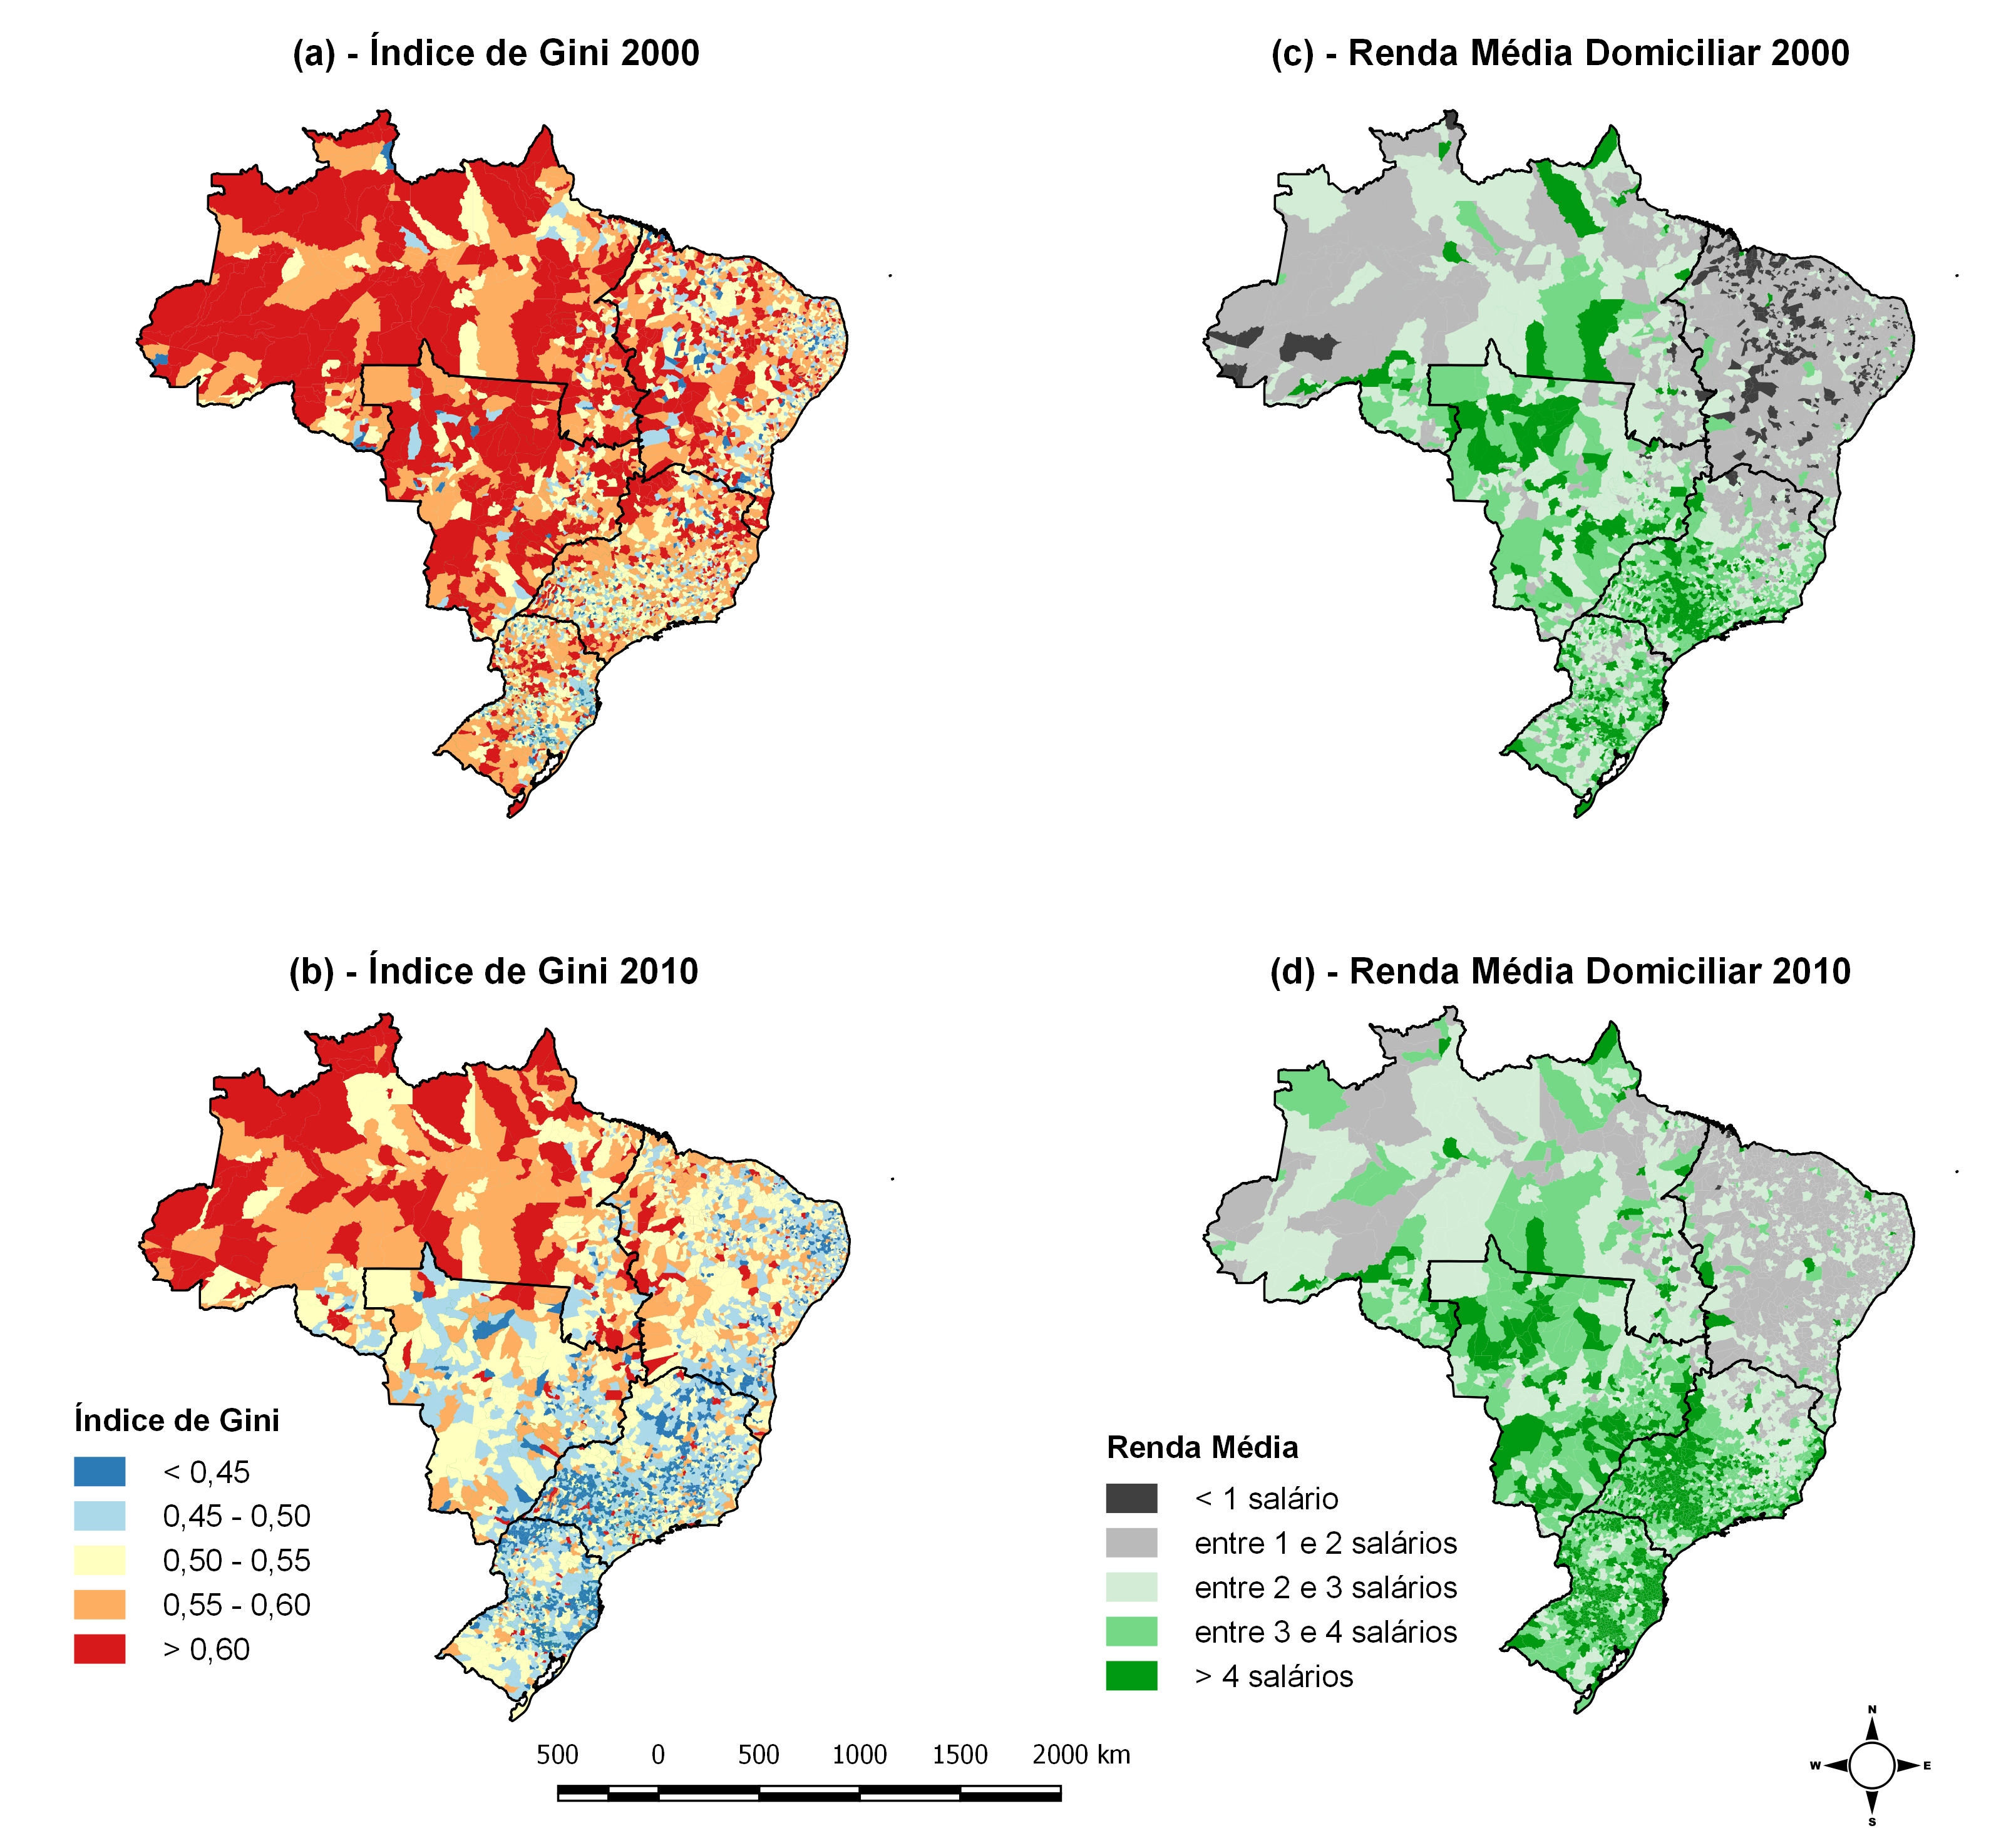
\includegraphics[width=\textwidth]{figs/cap04_mapa_gini_renda.png}
    \caption*{\footnotesize{Fonte: Elaborado pelo autor}}
    \label{fig:cap04:ginicidades}
\end{figure}

Do mesmo modo, as subfiguras \ref{fig:cap04:ginicidades}(c) e \ref{fig:cap04:ginicidades}(d) ilustram os rendimentos médios domiciliares (valores deflacionados para outubro de 2010 pelo INCP) dos municípios brasileiros nos anos de 2000 e 2010. Acerca desses mapas, é evidente o contraste existente no país, no qual cidades das regiões sul, sudeste e centro-oeste apresentam índices de renda média superiores aos demais municípios do norte e nordeste. 

Quantificando esses resultados, aproximadamente 82\% das cidades tiveram redução no coeficiente, sendo que 25\% dessas tiveram uma diminuição acima de 0,1 para o indicador. Observando as subfiguras \ref{fig:cap04:ginicidades}(a) e \ref{fig:cap04:ginicidades}(b) ressalta-se que esses dados de redução não apresentaram tanto impacto nos municípios da região norte em relação as demais regiões. Além disso, os índices de rendimento médio domiciliar para esta região se mantiveram baixo em ambos os anos analisados, evidenciando dessa forma a necessidade de atenção especial para essas cidades no âmbito de políticas públicas.

Analisando a região nordeste, é notória a redução do indicador acerca dos seus municípios. Todavia, realizando uma avaliação comparativa entre índice de Gini e rendimento médio domiciliar, observa-se que embora a região apresente uma melhora na métrica, seus valores de renda média apresentam-se baixos, ou seja, embora a distribuição de renda apresente aparência igualitária a mesma é nivelada por valores baixos em relação a cidades das regiões Sul, Sudeste e Centro-Oeste. 

\pagebreak

Posteriormente, foi analisado o impacto da parcela de aposentadorias e pensões acerca dos resultados encontrados para o índice de Gini nas cidades e estados brasileiros. Primeiramente, optou-se por examinar a sua participação percentual acerca do rendimento mensal per capita de cada unidade federativa do Brasil, podendo ser observado na Figura~\ref{fig:cap04:aposen_pensao_estados}.

Examinando os resultados encontrados, percebe-se que essa parcela tem importante participação no rendimento mensal per capita, com médias estaduais de 15,36\% e 17,63\% para 2000 e 2010 respectivamente. Nota-se também que apenas as unidades federativas do Amapá e do Distrito Federal não tiveram uma variação percentual positiva no ano de 2010 em relação aos dados de 2000, evidenciando uma crescente presença desses benefícios acerca da economia nacional.

\begin{figure}[!ht]
    \centering
    \caption{Participação percentual das rendas de aposentadorias e pensões no total dos rendimentos per capita das unidades federativas brasileiras, 2000 e 2010}
    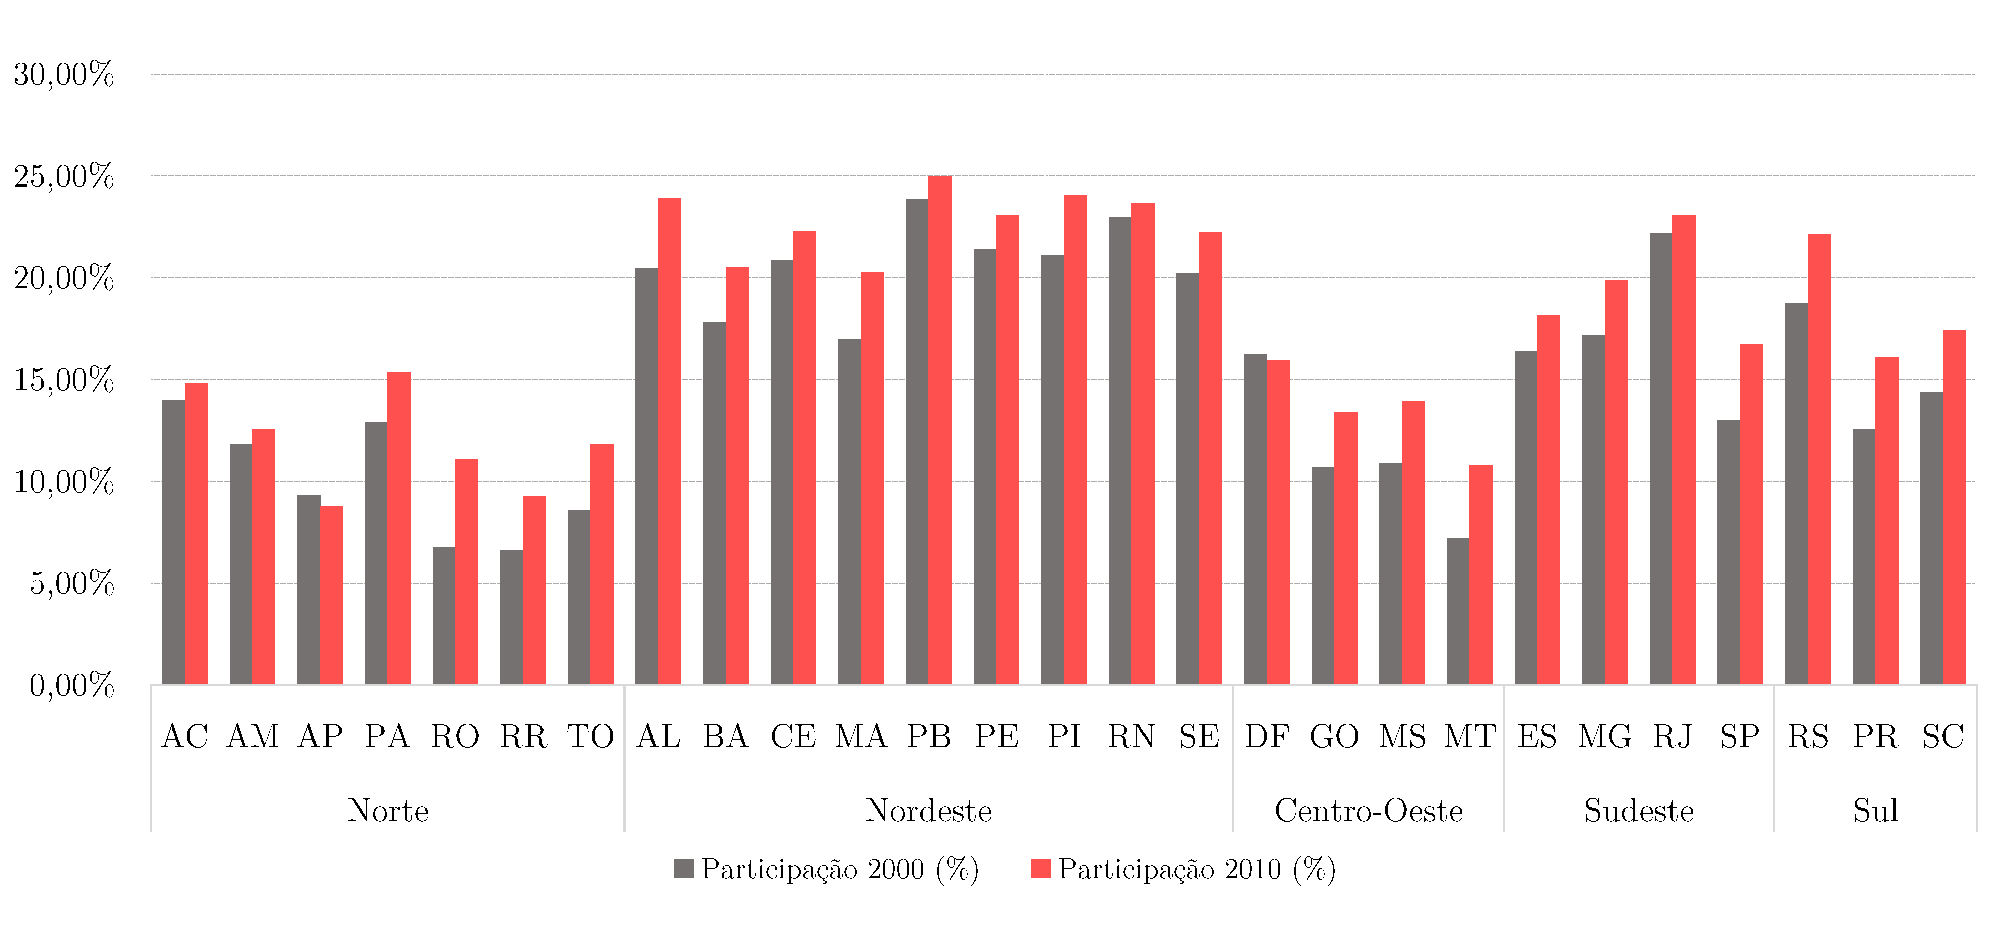
\includegraphics[width=\textwidth]{figs/cap04_aposen_pensao_estados.pdf}
    \caption*{\footnotesize{Fonte: Elaborado pelo autor}}
    \label{fig:cap04:aposen_pensao_estados}
\end{figure}

Em relação a evolução da participação total da parcela entre 2000 e 2010, destacam-se os estados de RO (Rondônia), RR (Roraima) e MT, com uma variação percentual positiva acima de 40\%. Além disso, os estados da região nordeste ganham atenção especial nessa análise, uma vez que em todos as aposentadorias e pensões representam pelo menos 1/5 de todo o rendimento per capita da população. Em escala municipal, a participação desses benefícios no rendimento da população é ainda mais impactante, com aproximadamente 45\% das cidades (2.465 municípios) apresentando pelo menos 1/3 dos rendimentos per capita provenientes dos benefícios citados no ano de 2010.  

Conforme descrito na Equação~\ref{eq:2.13} da Metodologia, a progressividade ($\pi_h$), ou razão concentração, é uma métrica utilizada para aferir a contribuição de uma parcela de rendimento no aumento ou diminuição da desigualdade de renda de uma população. Estudos realizados na literatura identificam que a parcela de aposentadorias e pensões contribui para a concentração de renda no Brasil \cite{cap02_ref22}.

Entretanto, analisando a Tabela~\ref{tab:cap04:progressividadeestados} observa-se que a categoria até um salário mínimo apresenta caráter progressivo ($\pi_h > 0$), colaborando para a diminuição da concentração de renda, para todos os estados brasileiros em ambos os anos examinados. Em contrapartida, as aposentadorias e pensões acima de um salário mínimo se mostram regressivas ($\pi_h < 0$) em todos os estados, indicando uma participação dessa parcela para o aumento da concentração de renda no Brasil.

\begin{table}[!ht]
    \caption{Progressividade ($\pi_h$) da parcela de rendimentos de aposentadorias e pensões por categorias para os estados brasileiros, 2000 e 2010}
    \renewcommand{\arraystretch}{1.4}
    \resizebox{\textwidth}{!}{
    \begin{tabular}{lccccccccc}
    \Xhline{2pt}
     & AC & AL & AM & AP & BA & CE & DF & ES & GO \\ \cline{2-10} 
    até um salário - 2000 & {\color[HTML]{3531FF} 0,8904} & {\color[HTML]{3531FF} 0,7139} & {\color[HTML]{3531FF} 0,9482} & {\color[HTML]{3531FF} 0,9839} & {\color[HTML]{3531FF} 0,7086} & {\color[HTML]{3531FF} 0,7085} & {\color[HTML]{3531FF} 1,2129} & {\color[HTML]{3531FF} 0,9615} & {\color[HTML]{3531FF} 0,9554} \\
    até um salário - 2010 & {\color[HTML]{3531FF} 0,7168} & {\color[HTML]{3531FF} 0,5275} & {\color[HTML]{3531FF} 0,7288} & {\color[HTML]{3531FF} 0,6726} & {\color[HTML]{3531FF} 0,5609} & {\color[HTML]{3531FF} 0,4856} & {\color[HTML]{3531FF} 1,1914} & {\color[HTML]{3531FF} 0,8210} & {\color[HTML]{3531FF} 0,7927} \\
    acima de um salário - 2000 & {\color[HTML]{FE0000} -0,1043} & {\color[HTML]{FE0000} -0,2503} & {\color[HTML]{FE0000} -0,1719} & {\color[HTML]{FE0000} -0,1718} & {\color[HTML]{FE0000} -0,2289} & {\color[HTML]{FE0000} -0,2524} & {\color[HTML]{FE0000} -0,1387} & {\color[HTML]{FE0000} -0,1734} & {\color[HTML]{FE0000} -0,1819} \\
    acima de um salário - 2010 & {\color[HTML]{FE0000} -0,2019} & {\color[HTML]{FE0000} -0,2878} & {\color[HTML]{FE0000} -0,2334} & {\color[HTML]{FE0000} -0,1781} & {\color[HTML]{FE0000} -0,2588} & {\color[HTML]{FE0000} -0,2866} & {\color[HTML]{FE0000} -0,1349} & {\color[HTML]{FE0000} -0,2130} & {\color[HTML]{FE0000} -0,2293} \\ \Xhline{2pt}
     & MA & MG & MS & MT & PA & PB & PE & PI & PR \\ \cline{2-10} 
    até um salário - 2000 & {\color[HTML]{3531FF} 0,5486} & {\color[HTML]{3531FF} 0,9630} & {\color[HTML]{3531FF} 0,9998} & {\color[HTML]{3531FF} 1,0264} & {\color[HTML]{3531FF} 0,8381} & {\color[HTML]{3531FF} 0,6896} & {\color[HTML]{3531FF} 0,8255} & {\color[HTML]{3531FF} 0,5637} & {\color[HTML]{3531FF} 1,0244} \\
    até um salário - 2010 & {\color[HTML]{3531FF} 0,4037} & {\color[HTML]{3531FF} 0,8138} & {\color[HTML]{3531FF} 0,8721} & {\color[HTML]{3531FF} 0,8693} & {\color[HTML]{3531FF} 0,5670} & {\color[HTML]{3531FF} 0,5435} & {\color[HTML]{3531FF} 0,6020} & {\color[HTML]{3531FF} 0,4403} & {\color[HTML]{3531FF} 0,9043} \\
    acima de um salário - 2000 & {\color[HTML]{FE0000} -0,2847} & {\color[HTML]{FE0000} -0,1635} & {\color[HTML]{FE0000} -0,1530} & {\color[HTML]{FE0000} -0,1602} & {\color[HTML]{FE0000} -0,2124} & {\color[HTML]{FE0000} -0,2715} & {\color[HTML]{FE0000} -0,2097} & {\color[HTML]{FE0000} -0,2628} & {\color[HTML]{FE0000} -0,1048} \\
    acima de um salário - 2010 & {\color[HTML]{FE0000} -0,2713} & {\color[HTML]{FE0000} -0,2329} & {\color[HTML]{FE0000} -0,2118} & {\color[HTML]{FE0000} -0,2173} & {\color[HTML]{FE0000} -0,2612} & {\color[HTML]{FE0000} -0,2727} & {\color[HTML]{FE0000} -0,2638} & {\color[HTML]{FE0000} -0,2619} & {\color[HTML]{FE0000} -0,1700} \\ \Xhline{2pt}
     & RJ & RN & RO & RR & RS & SC & SE & SP & TO \\ \cline{2-10} 
    até um salário - 2000 & {\color[HTML]{3531FF} 1,1402} & {\color[HTML]{3531FF} 0,8181} & {\color[HTML]{3531FF} 0,9099} & {\color[HTML]{3531FF} 0,9947} & {\color[HTML]{3531FF} 1,0494} & {\color[HTML]{3531FF} 1,0829} & {\color[HTML]{3531FF} 0,7038} & {\color[HTML]{3531FF} 1,1800} & {\color[HTML]{3531FF} 0,7877} \\
    até um salário - 2010 & {\color[HTML]{3531FF} 1,0064} & {\color[HTML]{3531FF} 0,5769} & {\color[HTML]{3531FF} 0,6994} & {\color[HTML]{3531FF} 0,7557} & {\color[HTML]{3531FF} 0,8935} & {\color[HTML]{3531FF} 0,9628} & {\color[HTML]{3531FF} 0,5785} & {\color[HTML]{3531FF} 1,0513} & {\color[HTML]{3531FF} 0,7044} \\
    acima de um salário - 2000 & {\color[HTML]{FE0000} -0,1008} & {\color[HTML]{FE0000} -0,2492} & {\color[HTML]{FE0000} -0,1095} & {\color[HTML]{FE0000} -0,1463} & {\color[HTML]{FE0000} -0,0955} & {\color[HTML]{FE0000} -0,0726} & {\color[HTML]{FE0000} -0,2429} & {\color[HTML]{FE0000} -0,0026} & {\color[HTML]{FE0000} -0,1976} \\
    acima de um salário - 2010 & {\color[HTML]{FE0000} -0,1711} & {\color[HTML]{FE0000} -0,2726} & {\color[HTML]{FE0000} -0,1775} & {\color[HTML]{FE0000} -0,1652} & {\color[HTML]{FE0000} -0,1675} & {\color[HTML]{FE0000} -0,1603} & {\color[HTML]{FE0000} -0,2710} & {\color[HTML]{FE0000} -0,1273} & {\color[HTML]{FE0000} -0,1873} \\ \Xhline{2pt}
    \end{tabular}}
    \label{tab:cap04:progressividadeestados}
    \caption*{\footnotesize{Fonte: Elaborado pelo autor.}}
\end{table}

\pagebreak

Na Figura~\ref{fig:cap04:progcidades} é exibida a situação da progressividade acerca dos municípios brasileiros. As subfiguras \ref{fig:cap04:progcidades}(a) e \ref{fig:cap04:progcidades}(c), correspondentes à parcela até um salário mínimo para 2000 e 2010, respectivamente, demonstram que o padrão exibido na análise das unidades federativas brasileiras se repete em quase todo território nacional, onde grande parte dos municípios apresentam caráter progressivo ($\pi_h > 0$) para a categoria. Destacam-se as cidades das regiões Norte, Sul, Sudeste, Centro-Oeste para 2000 e Sul, Sudeste e Centro-Oeste para 2010, as quais apresentam maiores índices de progressividade.

\begin{figure}[!ht]
    \centering
    \caption{Progressividade ($\pi_h$) da parcela de rendimentos de aposentadorias e pensões por categorias para os municípios brasileiros, 2000 e 2010}
    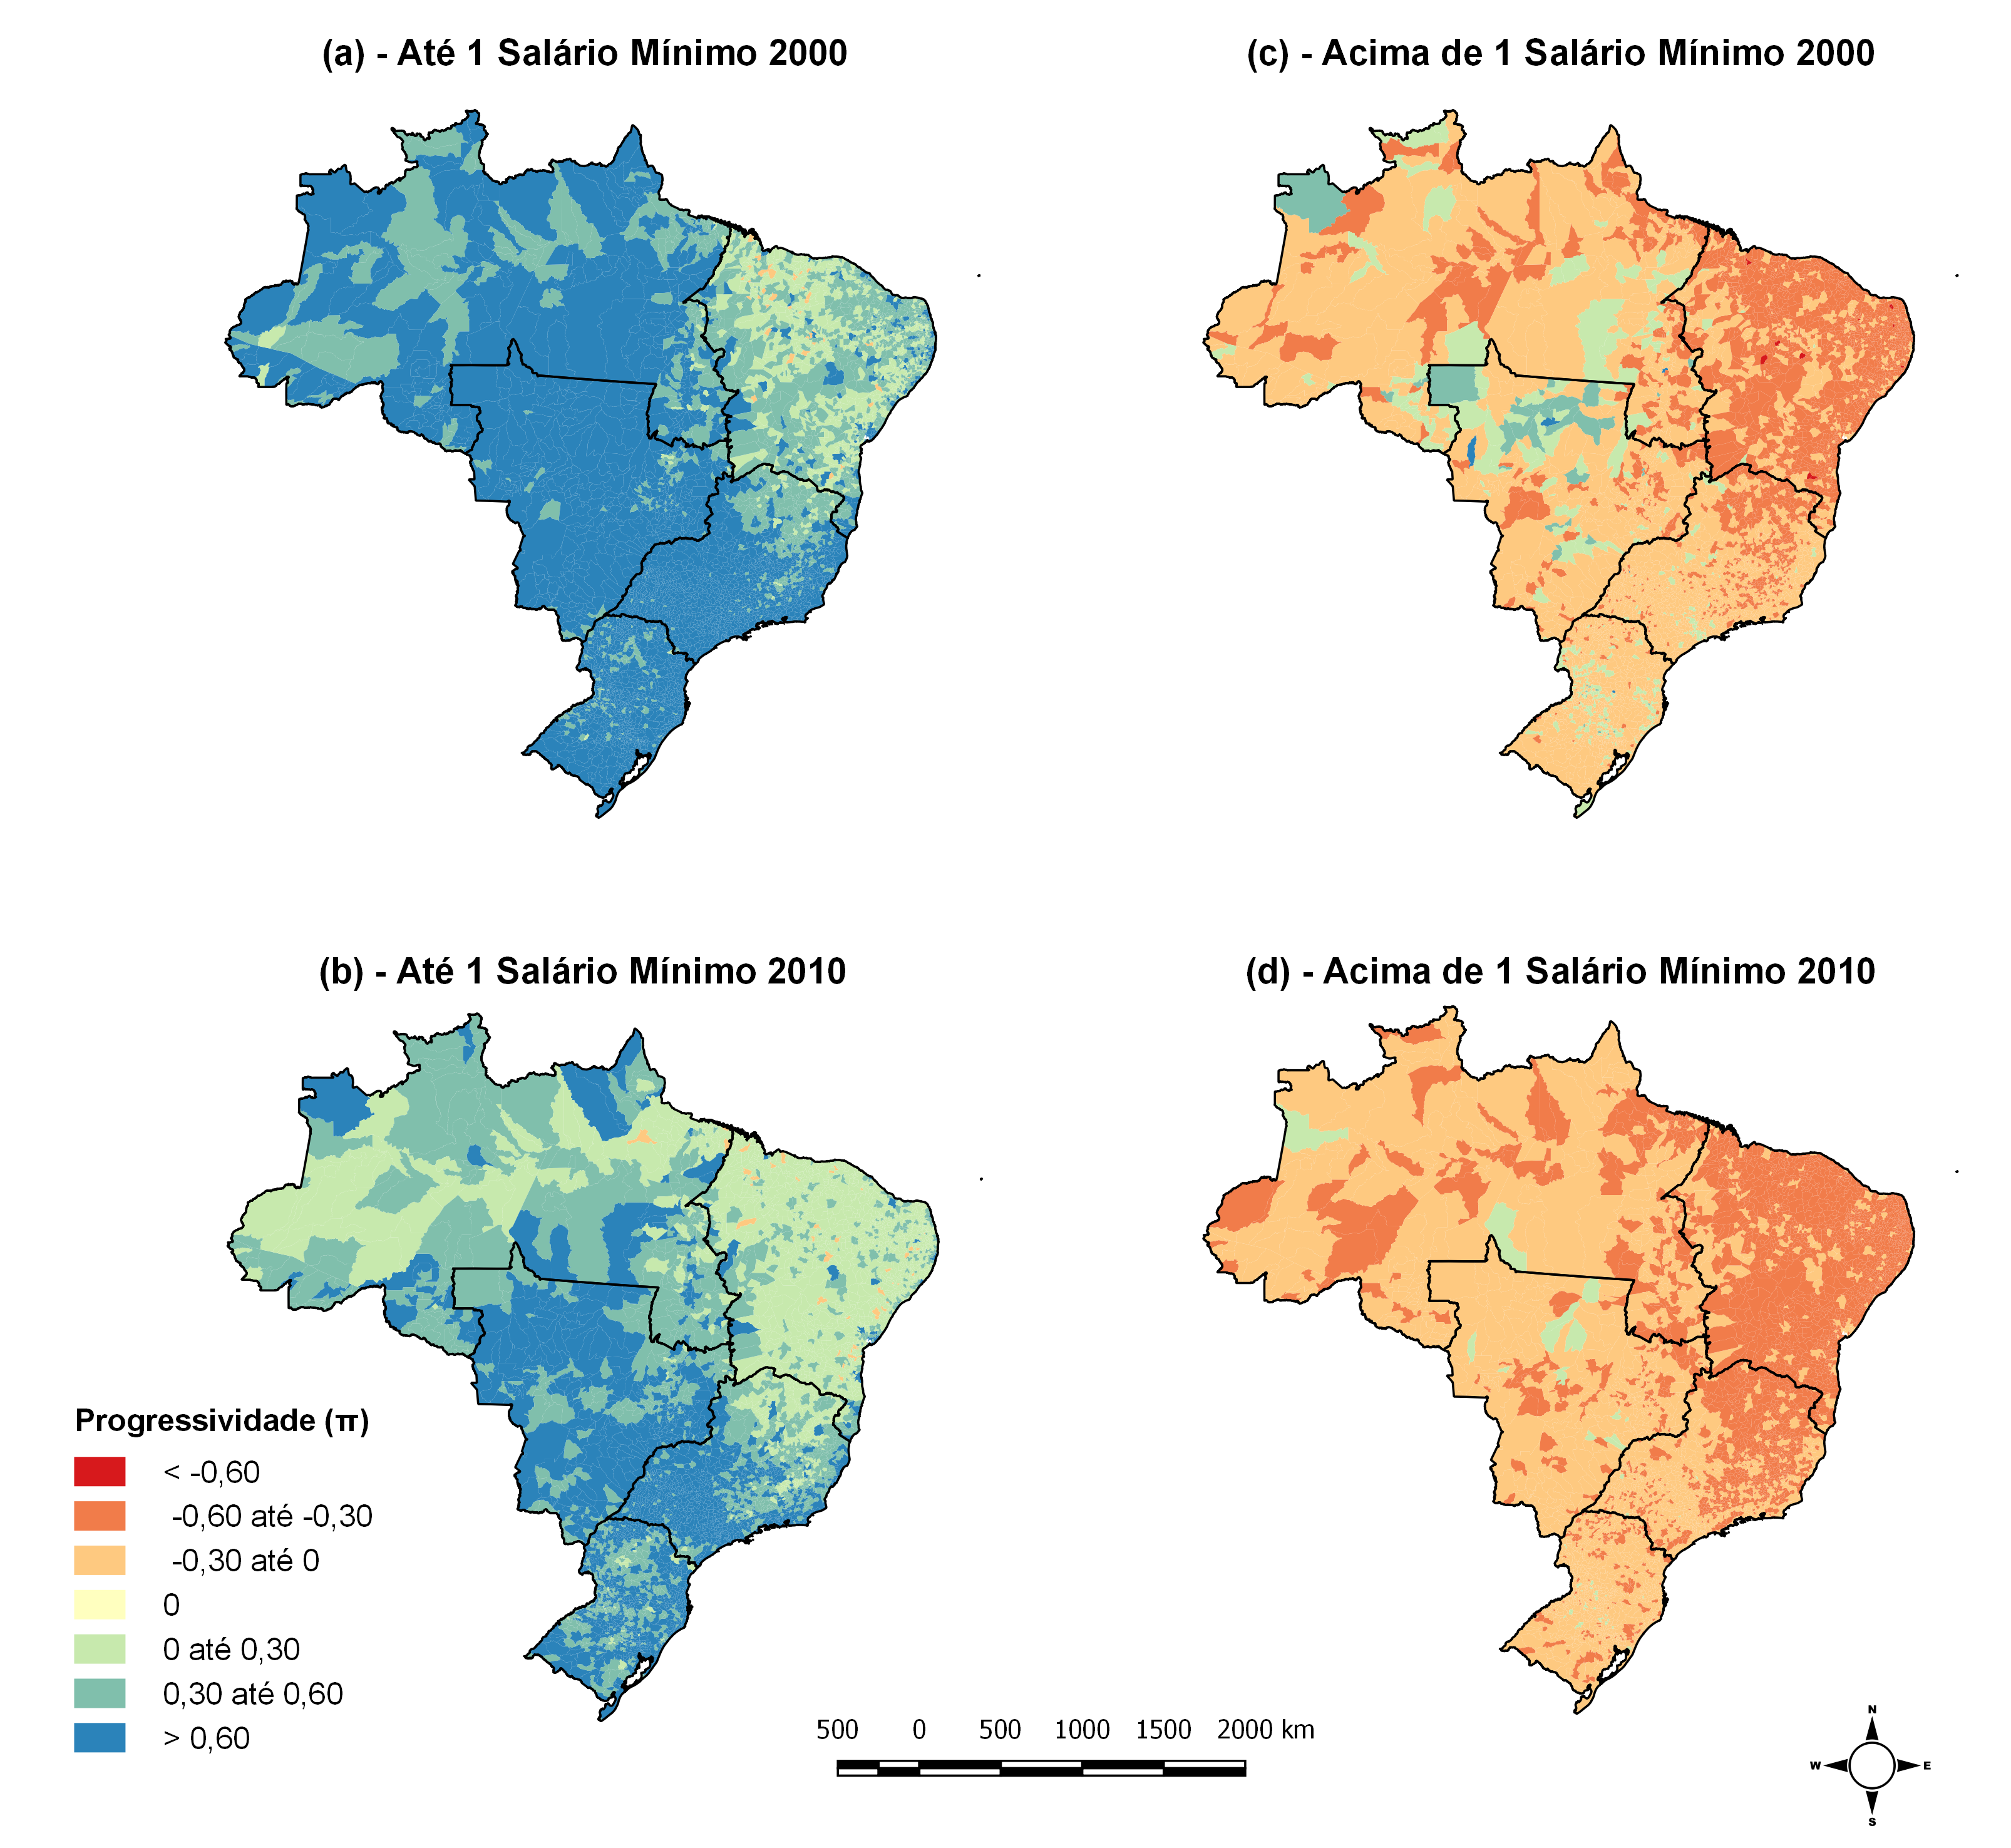
\includegraphics[width=\textwidth]{figs/cap04_mapa_prog_cidades.png}
    \caption*{\footnotesize{Fonte: Elaborado pelo autor}}
    \label{fig:cap04:progcidades}
\end{figure}

Do mesmo modo, as subfiguras \ref{fig:cap04:progcidades}(b) e \ref{fig:cap04:progcidades}(d) ilustram as situações das progressividades para as parcelas de aposentadorias e pensões acima de um salário mínimo nos anos de 2000 e 2010 respectivamente. O caráter regressivo ($\pi_h < 0$) observado em todos as unidades federativas para essa variável se repete acerca de grande parte dos municípios brasileiros, demostrando a importante participação dessa categoria no aumento da desigualdade de rendimentos no país.

As cidades da região nordeste destacam-se em relação as demais regiões, apresentando valores ligeiramente negativos para o indicador na categoria acima de um salário mínimo, e índices baixos na parcela de até um salário em ambos os anos analisados. Tal resultado indica que embora grande parte dos rendimentos nesta região sejam proveniente dessa categoria de benefício, conforme indicado na Figura~\ref{fig:cap04:progcidades}, possivelmente as aposentadorias e pensões acima de um salário estão concentradas na menor parcela de beneficiários, colaborando diretamente para concentração de renda existente nesses municípios. 

Posteriormente, foi avaliada a interdependência estatística existente entre o índice de Gini, os percentuais de participação dos benefícios acerca da composição de renda per capita e as progressividades resultantes para aposentadorias e pensões. Dessa forma, utilizando o coeficiente de Pearson, foram desenvolvidas as matrizes de correlação dos atributos analisados para os anos de 2000 e 2010 exibidas nas Figuras~\ref{fig:cap04:matrixcorr}(a) e \ref{fig:cap04:matrixcorr}(b) respectivamente.

\begin{figure}[!h]
    \centering
    \caption{Matrizes de correlação das variáveis. (a) 2000 (b) 2010}
    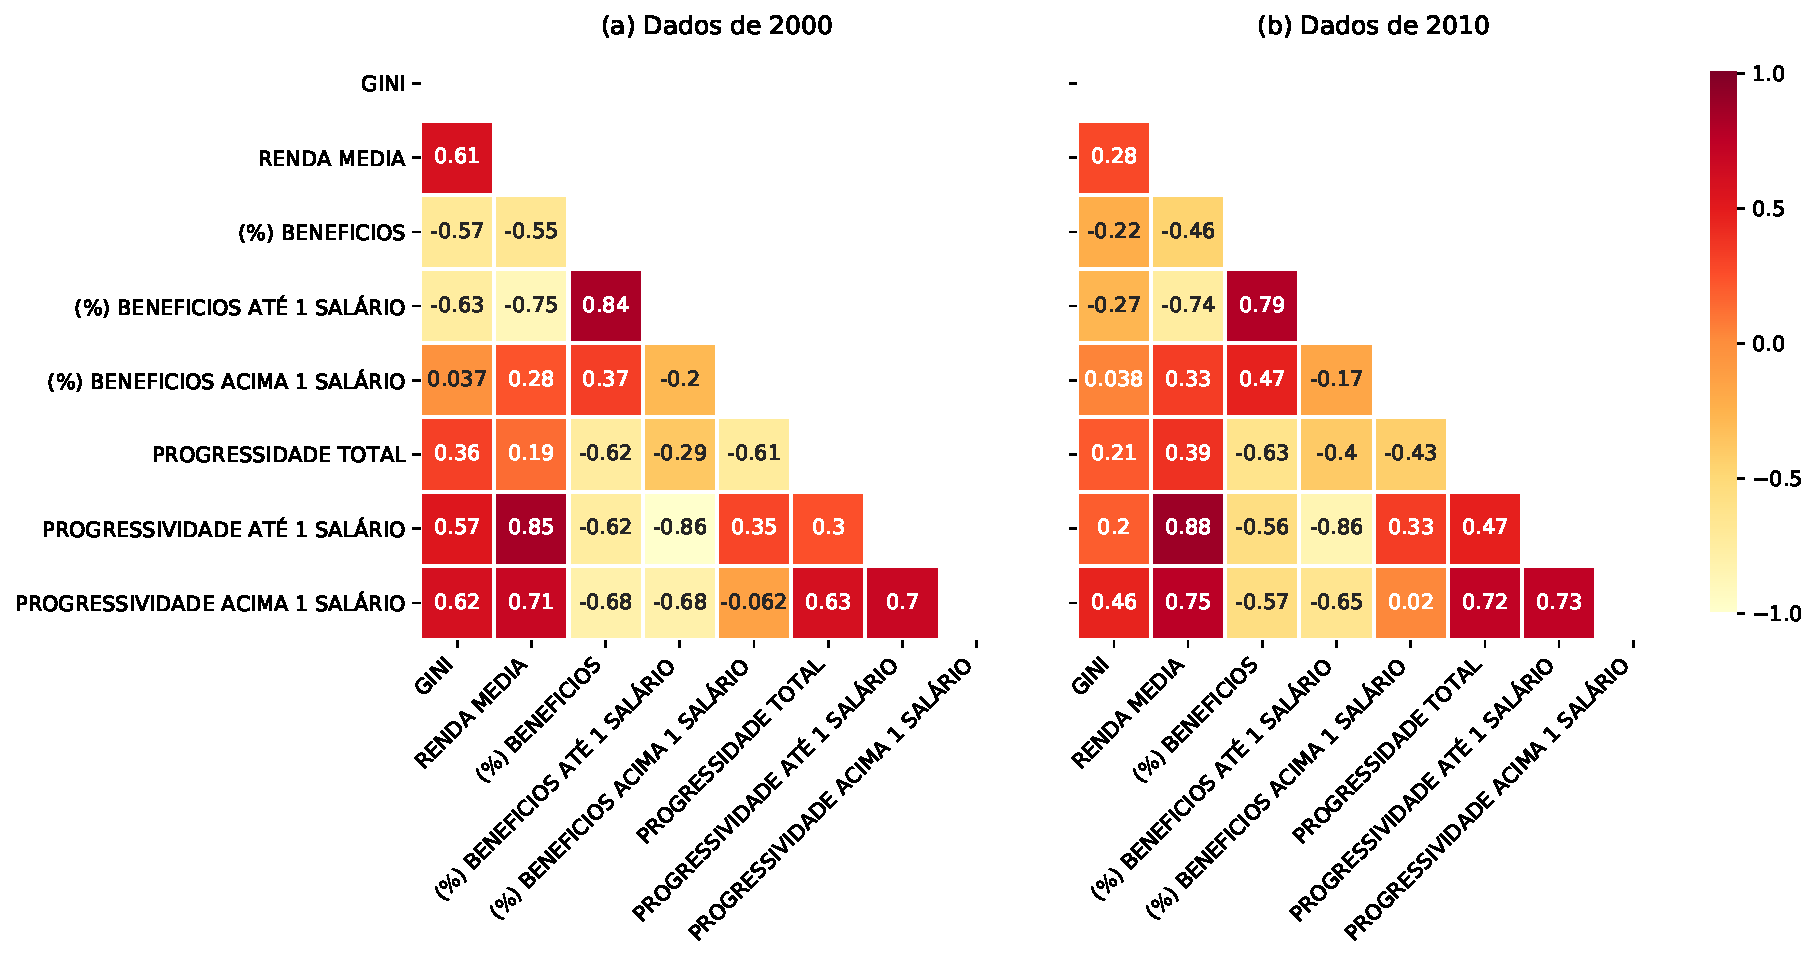
\includegraphics[width=\textwidth]{figs/cap04_corr_matrix.pdf}
    \caption*{\footnotesize{Fonte: Elaborado pelo autor}}
    \label{fig:cap04:matrixcorr}
\end{figure}

Avaliando a imagem, é possível observar uma diminuição na inter-relação existente entre a desigualdade de renda e as demais variáveis examinadas para o intervalo de tempo analisado. Destaca-se a correlação negativa existente entre o índice de Gini e o percentual de participação das aposentadorias e pensões - total e até um salário mínimo - na composição de renda da população. Tal fator indica uma tendencia inversamente proporcional entre as variáveis, ou seja, quanto maior taxa de participação dessa categoria acerca dos municípios brasileiros, menor será a desigualdade de distribuição de riquezas. 

No entanto, evidencia-se a interdependência negativa entre o percentual de participação dos benefícios e a renda média da população, pressupondo que embora essa categoria colabore para equalização de rendimentos, a mesma nivela os valores de renda por baixo. Por outro lado, a correlação existente entre as progressividades e a participação das aposentadorias e pensões demonstram, novamente, o importante papel que esses benefícios possuem na desigualdade de renda existente nos municípios. Todavia, destaca-se a importância de examinar variáveis geográficas, como a distancia das cidades em relação às metrópoles ou suas clientelas, afim de compreender melhor as interdependências existentes.

% --------------------------------------------------------------------------- %

\section{Considerações Finais}\label{cap04:conclusoes}

No presente estudo foi analisada a participação dos benefícios de aposentadorias e pensões na distribuição de renda per capita do Brasil (estados e municípios) nos anos de 2000 e 2010. A partir dos resultados demonstrados para o índice de Gini, conclui-se que embora haja uma heterogeneidade na sua distribuição acerca do território nacional, houve uma melhora no parâmetro, tanto a nível estadual quanto municipal, entre os anos analisados. Paralelamente, perante o cenário relatado anteriormente, o qual expõe a extensão da longevidade da população brasileira e o impacto econômico gerado pelo aumento na distribuição das aposentadorias e pensões, foi comprovado um acréscimo na participação percentual dessa parcela no total de rendimento per capita em todos os estados brasileiros.

No entanto, quando analisadas as participações das aposentadorias e pensões, dividindo-as em categorias (até um salário e acima de um salário), os resultados demonstraram que ambas têm papel divergente em sua contribuição para a concentração de renda. Com um padrão se repetindo em todos os estados – e maioria das cidades brasileiras –, os benefícios acima de um salário apresentaram caráter regressivo ($ \pi_h < 0$), colaborando para um aumento do índice de Gini, destacando-se a maior parte dos municípios do nordeste. Por outro lado, a categoria de benefícios até um salário demonstrou caráter progressivo ($\pi_h > 0$) em todo o país, colaborando para uma desconcentração de renda e decréscimo do índice de Gini.  

Com isso, identifica-se que embora as aposentadorias e pensões colaborem para a concentração de renda no Brasil, conforme apresentado por \cite{cap04_ref7, cap04_ref8, cap04_ref9} , tal fator apresenta caráter contraditório ao segmentarmos os benefícios em diferentes faixas salariais, uma vez que cada categoria colabora de forma diferente acerca da distribuição de renda. Dessa forma, correlacionando tal fator à heterogeneidade que o índice de Gini apresenta no cenário brasileiro, é possível vislumbrar discussões e análises cada vez mais complexas que objetivem equalizar as variáveis relacionadas a essa problemática.

Contudo, destaca-se que relatórios e estudos recentes apontam uma variação positiva para o coeficiente de Gini nos últimos anos, fator diretamente relacionado a crise econômica nacional a qual registrou uma queda de aproximadamente 9\% no PIB entre 2014 e 2016 \cite{cap04_ref19}. Dessa forma, evidencia-se a necessidade de pesquisas com dados atualizados acerca dos municípios brasileiros a fim de mensurar a real situação de distribuição de renda do país, além do impacto que as aposentadorias e pensões causam nessa. Entretanto, os valores de rendimento domiciliar (e dos benefícios que os compõe), a nível municipal, são informações disponibilizadas apenas pelo censo demográfico, impossibilitando a realização de tais análises no presente momento.

Diante disso, como trabalhos futuros, propõem-se a replicação do atual estudo utilizando os dados futuramente disponibilizados pelo IBGE relacionados ao censo demográfico de 2020, a exploração de outros indicadores econômico-sociais (como por exemplo o índice de \textit{Theil}), a aplicação técnicas de inteligência computacional para a extração de novos \textit{insights} acerca da problemática e a utilização de métodos estatísticos espaciais (como o Índice de Moran \cite{cap04_ref20}) a fim de compreender melhor a autocorrelação existente na dispersão das variáveis entre os municípios.
